\section{ROS} \label{sec:ros}
ROS (Robot Operating System) es un conjunto de herramientas y bibliotecas que permite desarrollar software para robots de forma modular y distribuida. Aunque su nombre incluye la palabra "sistema operativo", en realidad funciona como una capa intermedia que facilita la comunicación entre los diferentes componentes de un robot, como sensores, actuadores, nodos de procesamiento y simuladores \cite{ros2-understanding-topics}.

En la Figura~\ref{fig:rosconcepts} se muestra un diagrama de comunicación típico en ROS. En este se pueden ver los principales elementos del sistema: nodos, que ejecutan tareas específicas; temas (topics), que permiten el envío de mensajes entre nodos de forma asincrónica; servicios, que permiten una comunicación tipo solicitud-respuesta entre nodos; y los propios mensajes, que son las estructuras de datos utilizadas en estas interacciones.

\begin{figure}[h]
	\centering
	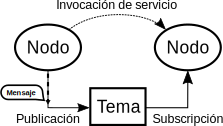
\includegraphics[width=0.5\linewidth]{img/ROS_concepts}
	\caption{Diagrama de comunicación de ROS}
	\label{fig:rosconcepts}
\end{figure}

\pagebreak[4]  

\subsection{Nodo (Node)}
En ROS, un nodo es una unidad básica de procesamiento que realiza una tarea específica dentro del sistema robótico. Por ejemplo, un nodo puede encargarse de leer sensores, controlar motores o realizar cálculos. Los nodos se comunican entre sí mediante mensajes, y pueden ser escritos en lenguajes como Python o C++. Durante las prácticas, se utilizaron nodos simples como el de \textit{turtlesim}, el cual simula una tortuga que se puede mover con comandos enviados desde otro nodo.

\subsection{Tema (Topic)}
Los temas (topics) son canales de comunicación por los cuales los nodos publican y reciben mensajes. Esta comunicación es asincrónica y sigue un modelo de publicación-suscripción. Por ejemplo, un nodo puede publicar la posición de un sensor en un topic llamado \texttt{/sensor\_data}, mientras que otro nodo se suscribe a ese topic para procesar la información. En el caso de \textit{turtlesim}, se utiliza el topic \texttt{/turtle1/cmd\_vel} para enviarle velocidades a la tortuga virtual.

\subsection{Mensaje (Message)}
Los mensajes en ROS son estructuras de datos que contienen la información enviada a través de los temas. Pueden ser tan simples como un número o más complejos, como coordenadas tridimensionales o imágenes. Cada mensaje está definido por un tipo específico y debe coincidir entre el publicador y el suscriptor. En las pruebas realizadas, se enviaban mensajes tipo \texttt{geometry\_msgs/Twist} para mover a la tortuga virtual.

\subsection{Servicio (Service)}
Los servicios permiten una comunicación síncrona entre nodos. A diferencia de los temas, los servicios funcionan como una llamada y respuesta: un nodo hace una petición (request) y otro nodo responde (response). Se usan para operaciones que necesitan una respuesta inmediata, como pedir una acción específica. Por ejemplo, en \textit{turtlesim} existe el servicio \texttt{/clear} que borra el rastro de la tortuga al ser llamado.

\subsection{Gazebo}
Gazebo es un simulador 3D que se puede integrar con ROS para probar robots en entornos virtuales antes de llevarlos al mundo real. Permite simular sensores, física, objetos y ambientes. En el proyecto, se utilizó Gazebo junto con ROS para simular el comportamiento del robot, observar su movimiento y validar comandos enviados desde nodos. 

\subsection{RViz}
RViz es una herramienta de visualización de ROS que permite ver datos en tiempo real como posiciones, trayectorias, sensores y modelos del robot. Es muy útil para verificar si los datos que se están generando o recibiendo son correctos. Aunque no fue el enfoque principal del proyecto, se llegó a usar RViz para observar el modelo del robot y validar la información de sensores o movimientos generados desde los nodos.
